\paragraph{}Los procesos que intervienen en dicho módulo son los siguientes:

\begin{description}
 \item[Validar alumno] Constará de los procedimientos necesarios para que se
      validen los datos de acceso permitiendo el acceso o no del alumno.
 \item[Procesar entrada] Constará de los procedimientos necesarios para que se
      mantenga la veracidad, integridad y consistencia de la base de datos así
      como la comprobación de la integridad de los datos introducidos por el
      alumno.
 \item[Gestionar información personal] Constará de los procedimientos necesarios
      para mantener toda la información personal del alumno en la base de datos.
 \item[Explotación del sistema]  Constará de los procedimientos necesarios para
      consultar datos de la aplicación.
 \item[Ayuda] Administra la documentación que sirve de ayuda en el manejo de
      esta aplicación.
 \item[Procesar salida] Constará de los procedimientos necesarios para que
      puedan ser visualizados los resultados de los procesos anteriores.
\end{description}

\paragraph{}La figura \ref{diagramaNivel2-Alumnos} muestra el nivel de
abstracción 2: Alumnos.

  \begin{figure}[!ht]
    \begin{center}
      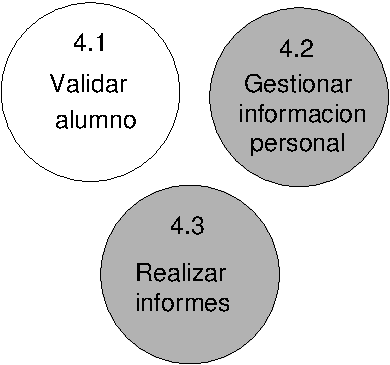
\includegraphics[]{08.Analisis_Funcional/8.2.DFDs/Niveles/Nivel2/Diagramas/nivel2-Alumnos.pdf}
      \caption{Nivel de abstracción 2: Alumnos.}
      \label{diagramaNivel2-Alumnos}
    \end{center}
  \end{figure}